%%%%%%%%%%%%%%%%%%%%%%%%%%%%%%%%%%%%

\section{Introduction to multiple regression}

%%%%%%%%%%%%%%%%%%%%%%%%%%%%%%%%%%%%

\begin{frame}
\frametitle{Multiple regression}

\begin{itemize}

\item Simple linear regression: Bivariate - two variables: $y$ and $x$

\item Multiple linear regression: Multiple variables: $y$ and $x_1, x_2, \cdots$

\end{itemize}

\end{frame}

%%%%%%%%%%%%%%%%%%%%%%%%%%%%%%%%%%%%

\subsection{Indicator and categorical variables as predictors}

%%%%%%%%%%%%%%%%%%%%%%%%%%%%%%%%%%%

\begin{frame}
\frametitle{Poverty vs. region (east, west)}


\[ \widehat{poverty} = 11.17 + 0.38 \times west \]

\begin{itemize}

\item Explanatory variable: region, \hl{reference level:} east

\item \hl{Intercept:} The estimated average poverty percentage in eastern states is 11.17\%
\pause
\begin{itemize}
\item This is the value we get if we plug in \orange{0} for the explanatory variable
\end{itemize}

\pause

\item \hl{Slope:} The estimated average poverty percentage in western states is 0.38\% higher than eastern states.
\pause
\begin{itemize}
\item Then, the estimated average poverty percentage in western states is 11.17 + 0.38 =  11.55\%.
\pause
\item This is the value we get if we plug in \orange{1} for the explanatory variable
\end{itemize}

\end{itemize}

\end{frame}

%%%%%%%%%%%%%%%%%%%%%%%%%%%%%%%%%%

\begin{frame}
\frametitle{Poverty vs. region (northeast, midwest, west, south)}

\pq{Which region (northeast, midwest, west, or south) is the reference level?}

{\small
\begin{center}
\begin{tabular}{rrrrr}
  \hline
 & Estimate & Std. Error & t value & Pr($>$$|$t$|$) \\ 
  \hline
(Intercept) & 9.50 & 0.87 & 10.94 & 0.00 \\ 
region4midwest & 0.03 & 1.15 & 0.02 & 0.98 \\ 
region4west & 1.79 & 1.13 & 1.59 & 0.12 \\ 
region4south & 4.16 & 1.07 & 3.87 & 0.00 \\ 
   \hline
\end{tabular}
\end{center}
}

\begin{enumerate}[(a)]
\solnMult{northeast}
\item midwest
\item west
\item south
\item cannot tell
\end{enumerate}

\end{frame}

%%%%%%%%%%%%%%%%%%%%%%%%%%%%%%%%%%%

\begin{frame}
\frametitle{Poverty vs. region (northeast, midwest, west, south)}

\pq{Which region (northeast, midwest, west, or south) has the lowest poverty percentage?}

{\small
\begin{center}
\begin{tabular}{rrrrr}
  \hline
 & Estimate & Std. Error & t value & Pr($>$$|$t$|$) \\ 
  \hline
(Intercept) & 9.50 & 0.87 & 10.94 & 0.00 \\ 
region4midwest & 0.03 & 1.15 & 0.02 & 0.98 \\ 
region4west & 1.79 & 1.13 & 1.59 & 0.12 \\ 
region4south & 4.16 & 1.07 & 3.87 & 0.00 \\ 
   \hline
\end{tabular}
\end{center}
}

\begin{enumerate}[(a)]
\solnMult{northeast}
\item midwest
\item west
\item south
\item cannot tell
\end{enumerate}

\end{frame}

%%%%%%%%%%%%%%%%%%%%%%%%%%%%%%%%%%%%

\subsection{Including and assessing many variables in a model}

%%%%%%%%%%%%%%%%%%%%%%%%%%%%%%%%%%%%

\begin{frame}
\frametitle{Weights of books}

\twocol{0.6}{0.4}{
{\footnotesize
\begin{center}
\begin{tabular}{rrrc}
  \hline
 & weight (g) & volume (cm$^\text{3}$) & cover \\ 
  \hline
1 & 800 & 885 & hc \\ 
  2 & 950 & 1016 & hc \\ 
  3 & 1050 & 1125 & hc \\ 
  4 & 350 & 239 & hc \\ 
  5 & 750 & 701 & hc \\ 
  6 & 600 & 641 & hc \\ 
  7 & 1075 & 1228 & hc \\ 
  8 & 250 & 412 & pb \\ 
  9 & 700 & 953 & pb \\ 
  10 & 650 & 929 & pb \\ 
  11 & 975 & 1492 & pb \\ 
  12 & 350 & 419 & pb \\ 
  13 & 950 & 1010 & pb \\ 
  14 & 425 & 595 & pb \\ 
  15 & 725 & 1034 & pb \\ 
   \hline
\end{tabular}
\end{center}
}}
{
\begin{center}
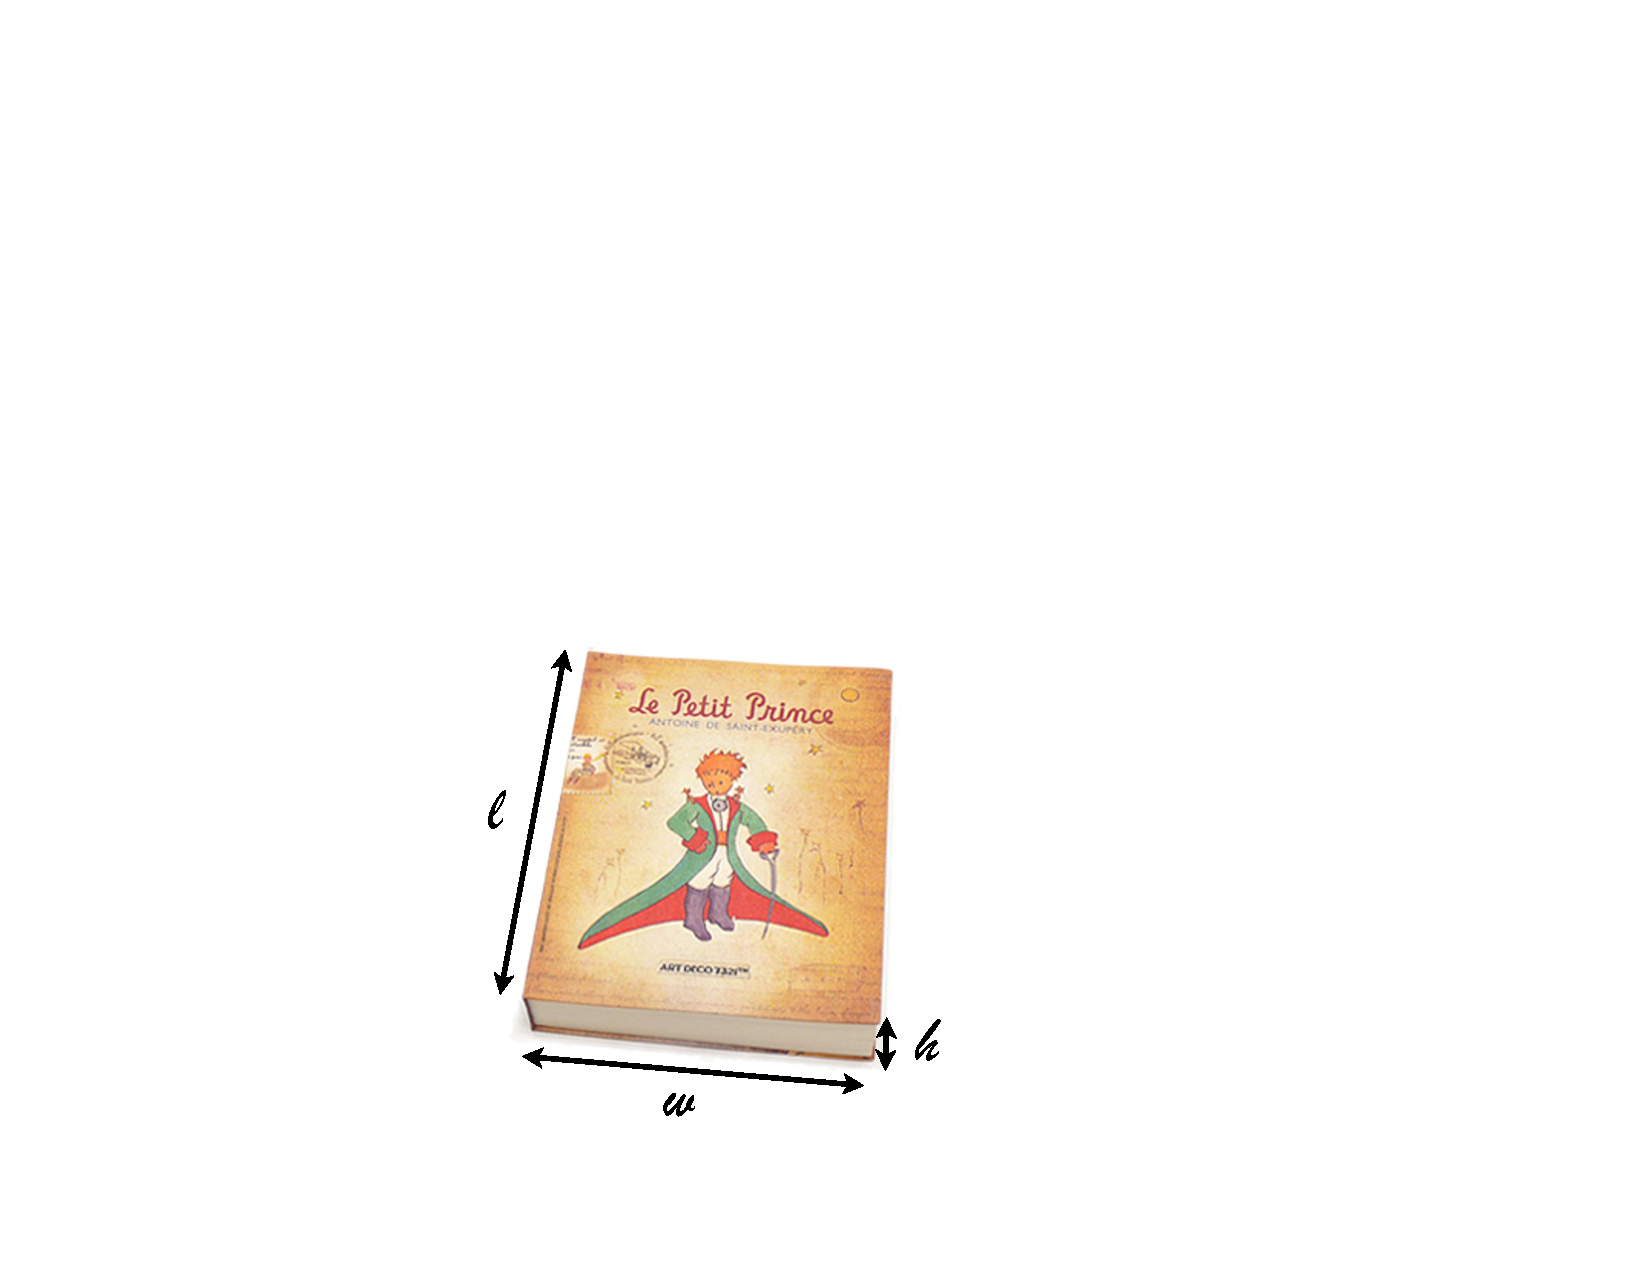
\includegraphics[width=0.7\textwidth]{9-1_intro_mlr/figures/books/book}
\end{center}
}

\ct{From: Maindonald, J.H. and Braun, W.J. (2nd ed., 2007) ``Data Analysis and Graphics Using R"}

\end{frame}

%%%%%%%%%%%%%%%%%%%%%%%%%%%%%%%%%%%

\begin{frame}
\frametitle{Weights of books (cont.)}

\twocol{0.45}{0.4}
{
\pq{{\small The scatterplot shows the relationship between weights and volumes of books as well as the regression output. Which of the below is correct?}}
}
{
\begin{center}
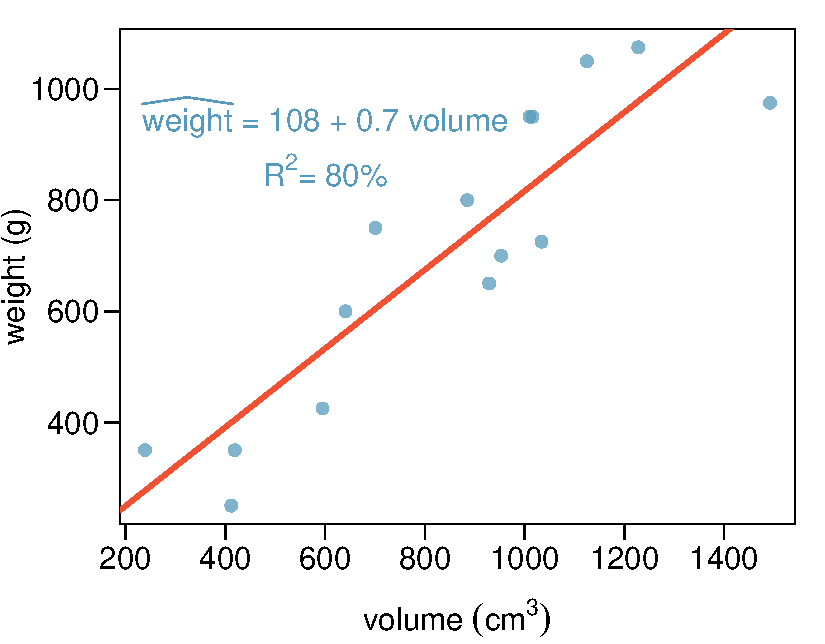
\includegraphics[width=\textwidth]{9-1_intro_mlr/figures/books/weight_volume}
\end{center}
}

\begin{enumerate}[(a)]
\item Weights of 80\% of the books can be predicted accurately using this model.
\solnMult{Books that are 10 cm$^\text{3}$ over average are expected to weigh 7 g over average.}
\item The correlation between weight and volume is $R = 0.80^2 = 0.64$.
\item The model underestimates the weight of the book with the highest volume.
\end{enumerate}

\end{frame}

%%%%%%%%%%%%%%%%%%%%%%%%%%%%%%%%%%%

\begin{frame}[fragile]
\frametitle{Modeling weights of books using volume}

{\small \textit{somewhat abbreviated output...}}

\begin{verbatim}
Coefficients:
             Estimate Std. Error t value Pr(>|t|)    
(Intercept) 107.67931   88.37758   1.218    0.245    
volume        0.70864    0.09746   7.271 6.26e-06


Residual standard error: 123.9 on 13 degrees of freedom
Multiple R-squared: 0.8026,	Adjusted R-squared: 0.7875 
F-statistic: 52.87 on 1 and 13 DF,  p-value: 6.262e-06 
\end{verbatim}

\end{frame}

%%%%%%%%%%%%%%%%%%%%%%%%%%%%%%%%%%%

\begin{frame}
\frametitle{Weights of hardcover and paperback books}

\dq{Can you identify a trend in the relationship between volume and weight of hardcover and paperback books?}

\soln{\only<2>{{\small Paperbacks generally weigh less than hardcover books after controlling for the book?s volume.}}}

\begin{center}
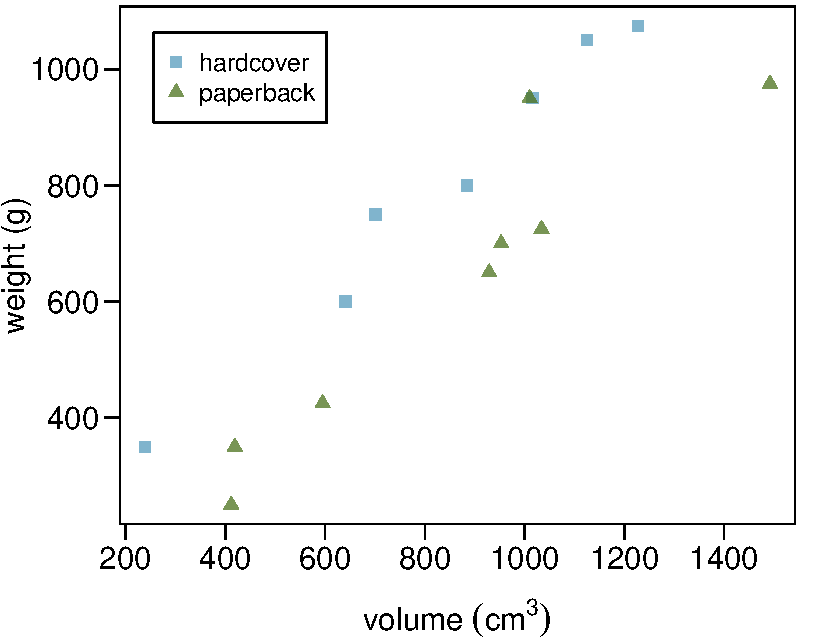
\includegraphics[width=0.6\textwidth]{9-1_intro_mlr/figures/books/weight_volume_cover}
\end{center}

\end{frame}

%%%%%%%%%%%%%%%%%%%%%%%%%%%%%%%%%%%

\begin{frame}[fragile]
\frametitle{Modeling weights of books using volume \underline{and} cover type}

\begin{verbatim}
Coefficients:
              Estimate Std. Error t value Pr(>|t|)    
(Intercept)  197.96284   59.19274   3.344 0.005841 ** 
volume         0.71795    0.06153  11.669  6.6e-08 ***
cover:pb    -184.04727   40.49420  -4.545 0.000672 ***


Residual standard error: 78.2 on 12 degrees of freedom
Multiple R-squared: 0.9275,	Adjusted R-squared: 0.9154 
F-statistic: 76.73 on 2 and 12 DF,  p-value: 1.455e-07 
\end{verbatim}

\end{frame}

%%%%%%%%%%%%%%%%%%%%%%%%%%%%%%%%%%%

\begin{frame}
\frametitle{Determining the reference level}

\pq{Based on the regression output below, which level of \var{cover} is the reference level? Note that \var{pb}: paperback.}

{\small
\begin{center}
\begin{tabular}{rrrrr}
  \hline
 & Estimate & Std. Error & t value & Pr($>$$|$t$|$) \\ 
  \hline
(Intercept) & 197.9628 & 59.1927 & 3.34 & 0.0058 \\ 
  volume & 0.7180 & 0.0615 & 11.67 & 0.0000 \\ 
  cover:pb & -184.0473 & 40.4942 & -4.55 & 0.0007 \\ 
   \hline
\end{tabular}
\end{center}
}

\begin{enumerate}[(a)]
\item paperback
\solnMult{hardcover}
\end{enumerate}

\end{frame}

%%%%%%%%%%%%%%%%%%%%%%%%%%%%%%%%%%%

\begin{frame}
\frametitle{Determining the reference level}

\pq{Which of the below correctly describes the roles of variables in this regression model?}

{\small
\begin{center}
\begin{tabular}{rrrrr}
  \hline
 & Estimate & Std. Error & t value & Pr($>$$|$t$|$) \\ 
  \hline
(Intercept) & 197.9628 & 59.1927 & 3.34 & 0.0058 \\ 
  volume & 0.7180 & 0.0615 & 11.67 & 0.0000 \\ 
  cover:pb & -184.0473 & 40.4942 & -4.55 & 0.0007 \\ 
   \hline
\end{tabular}
\end{center}
}

\begin{enumerate}[(a)]
\item response: weight, explanatory: volume, paperback cover
\item response: weight, explanatory: volume, hardcover cover
\item response: volume, explanatory: weight, cover type
\solnMult{response: weight, explanatory: volume, cover type}
\end{enumerate}

\end{frame}

%%%%%%%%%%%%%%%%%%%%%%%%%%%%%%%%%%%

\begin{frame}
\frametitle{Linear model}

{\small
\begin{center}
\begin{tabular}{rrrrr}
  \hline
 & Estimate & Std. Error & t value & Pr($>$$|$t$|$) \\ 
  \hline
(Intercept) & 197.96 & 59.19 & 3.34 & 0.01 \\ 
  volume & 0.72 & 0.06 & 11.67 & 0.00 \\ 
  cover:pb & -184.05 & 40.49 & -4.55 & 0.00 \\ 
   \hline
\end{tabular}
\end{center}
}

\pause

\[ \widehat{weight} = 197.96 + 0.72~volume - 184.05~cover:pb  \]

\pause

\begin{enumerate}

\item For \hl{hardcover} books: plug in \orange{0} for \var{cover}
\begin{eqnarray*}
\widehat{weight} &=& 197.96 + 0.72~volume - 184.05 \times \orange{0} \\
\pause
&=& 197.96 +  0.72~volume
\end{eqnarray*}

\pause

\item For \orange{paperback} books: plug in \orange{1} for \var{cover}
\begin{eqnarray*}
\widehat{weight} &=& 197.96 + 0.72~volume - 184.05 \times \orange{1} \\
\pause
&=& 13.91 +  0.72~volume
\end{eqnarray*}

\end{enumerate}

\end{frame}

%%%%%%%%%%%%%%%%%%%%%%%%%%%%%%%%%%%

\begin{frame}
\frametitle{Visualising the linear model}

\begin{center}
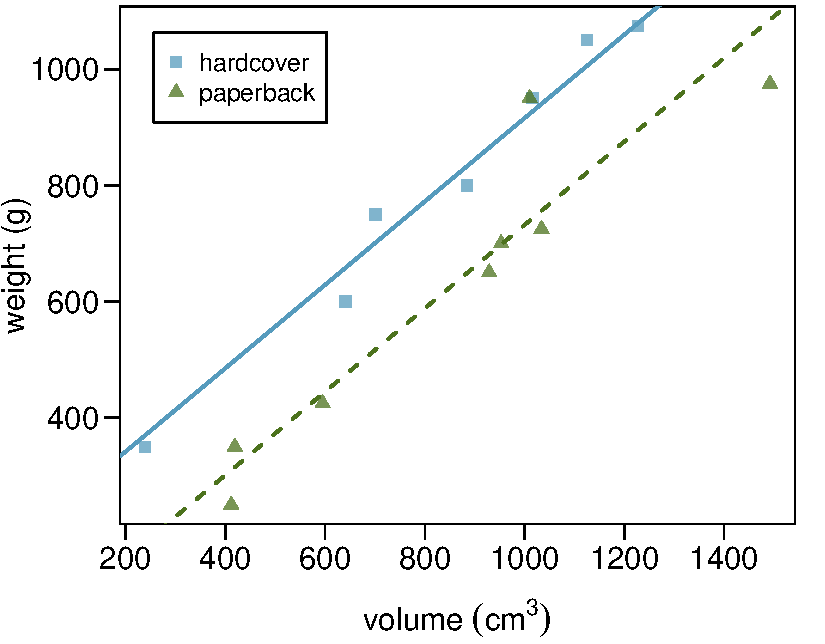
\includegraphics[width=0.8\textwidth]{9-1_intro_mlr/figures/books/weight_volume_cover_lines}
\end{center}

\end{frame}

%%%%%%%%%%%%%%%%%%%%%%%%%%%%%%%%%%%

\begin{frame}
\frametitle{Interpretation of the regression coefficients}

{\small
\begin{center}
\begin{tabular}{rrrrr}
  \hline
 & Estimate & Std. Error & t value & Pr($>$$|$t$|$) \\ 
  \hline
(Intercept) & 197.96 & 59.19 & 3.34 & 0.01 \\ 
  volume & 0.72 & 0.06 & 11.67 & 0.00 \\ 
  cover:pb & -184.05 & 40.49 & -4.55 & 0.00 \\ 
   \hline
\end{tabular}
\end{center}
}

\pause

\begin{itemize}

\item \hl{Slope of volume:} \underline{All else held constant}, books that are 1 more cubic centimeter in volume tend to weigh about 0.72 grams more.

\pause

\item \hl{Slope of cover:} \underline{All else held constant}, the model predicts that paperback books weigh 184 grams lower than hardcover books.

\pause

\item \hl{Intercept:} Hardcover books with no volume are expected on average to weigh 198 grams. \pause
\begin{itemize}
\item Obviously, the intercept does not make sense in context. It only serves to adjust the height of the line.
\end{itemize}

\end{itemize}

\end{frame}

%%%%%%%%%%%%%%%%%%%%%%%%%%%%%%%%%%%

\begin{frame}
\frametitle{Prediction}

\pq{Which of the following is the correct calculation for the predicted weight of a paperback book that is 600 cm$^3$?}

{\small
\begin{center}
\begin{tabular}{rrrrr}
  \hline
 & Estimate & Std. Error & t value & Pr($>$$|$t$|$) \\ 
  \hline
(Intercept) & 197.96 & 59.19 & 3.34 & 0.01 \\ 
  volume & 0.72 & 0.06 & 11.67 & 0.00 \\ 
  cover:pb & -184.05 & 40.49 & -4.55 & 0.00 \\ 
   \hline
\end{tabular}
\end{center}
}

\begin{enumerate}[(a)]
\solnMult{197.96 + 0.72 * 600 - 184.05 * 1} \soln{\only<2>{\orange{~$= 445.91$ grams}}}
\item 184.05 + 0.72 * 600 - 197.96 * 1
\item 197.96 + 0.72 * 600 - 184.05 * 0
\item 197.96 + 0.72 * 1 - 184.05 * 600
\end{enumerate}

\end{frame}

%%%%%%%%%%%%%%%%%%%%%%%%%%%%%%%%%%%

\begin{frame}
\frametitle{Another example: Modeling kid's test scores}

Predicting cognitive test scores of three- and four-year-old children using characteristics of their mothers. Data are from a survey of adult American women and their children - a subsample from the National Longitudinal Survey of Youth.

{\small
\begin{center}
\begin{tabular}{rrlrlr}
  \hline
 & kid\_score & mom\_hs & mom\_iq & mom\_work & mom\_age \\ 
  \hline
1 &  65 & yes & 121.12 & yes &  27 \\ 
  \vdots \\
  5 & 115 & yes & 92.75 & yes &  27 \\ 
  6 &  98 & no & 107.90 & no &  18 \\ 
  \vdots \\
  434 &  70 & yes & 91.25 & yes &  25 \\ 
   \hline
\end{tabular}
\end{center}
}

\vfill

{\tiny Gelman, Hill. \textit{Data Analysis Using Regression and Multilevel/Hierarchical Models}. (2007) Cambridge University Press.}

\end{frame}

%%%%%%%%%%%%%%%%%%%%%%%%%%%%%%%%%%%

\begin{frame}
\frametitle{Interpreting the slope}

\dq{What is the correct interpretation of the \underline{slope for mom's IQ}?}

{\small
\begin{center}
\begin{tabular}{rrrrr}
  \hline
 & Estimate & Std. Error & t value & Pr($>$$|$t$|$) \\ 
  \hline
(Intercept) & 19.59 & 9.22 & 2.13 & 0.03 \\ 
  mom\_hs:yes & 5.09 & 2.31 & 2.20 & 0.03 \\ 
  mom\_iq & 0.56 & 0.06 & 9.26 & 0.00 \\ 
  mom\_work:yes & 2.54 & 2.35 & 1.08 & 0.28 \\ 
  mom\_age & 0.22 & 0.33 & 0.66 & 0.51 \\ 
   \hline
\end{tabular}
\end{center}
}

$\:$ \\

\soln{\only<2>{All else held constant}, kids with mothers whose IQs are one point higher tend to score on average 0.56 points higher.}

\end{frame}

%%%%%%%%%%%%%%%%%%%%%%%%%%%%%%%%%%%

\begin{frame}
\frametitle{Interpreting the slope}

\dq{What is the correct interpretation of the \underline{intercept}?}

{\small
\begin{center}
\begin{tabular}{rrrrr}
  \hline
 & Estimate & Std. Error & t value & Pr($>$$|$t$|$) \\ 
  \hline
(Intercept) & 19.59 & 9.22 & 2.13 & 0.03 \\ 
  mom\_hs:yes & 5.09 & 2.31 & 2.20 & 0.03 \\ 
  mom\_iq & 0.56 & 0.06 & 9.26 & 0.00 \\ 
  mom\_work:yes & 2.54 & 2.35 & 1.08 & 0.28 \\ 
  mom\_age & 0.22 & 0.33 & 0.66 & 0.51 \\ 
   \hline
\end{tabular}
\end{center}
}

$\:$ \\

\soln{\only<2>{Kids whose moms haven't gone to HS, did not work during the first three years of the kid's life, have an IQ of 0 and are 0 yrs old are expected on average to score 19.59. Obviously, the intercept does not make any sense in context.}}

\end{frame}

%%%%%%%%%%%%%%%%%%%%%%%%%%%%%%%%%%%

\begin{frame}
\frametitle{Interpreting the slope}

\pq{What is the correct interpretation of the slope for \var{mom\_work}?}

{\scriptsize
\begin{center}
\begin{tabular}{rrrrr}
  \hline
 & Estimate & Std. Error & t value & Pr($>$$|$t$|$) \\ 
  \hline
(Intercept) & 19.59 & 9.22 & 2.13 & 0.03 \\ 
  mom\_hs:yes & 5.09 & 2.31 & 2.20 & 0.03 \\ 
  mom\_iq & 0.56 & 0.06 & 9.26 & 0.00 \\ 
  mom\_work:yes & 2.54 & 2.35 & 1.08 & 0.28 \\ 
  mom\_age & 0.22 & 0.33 & 0.66 & 0.51 \\ 
   \hline
\end{tabular}
\end{center}
}

All else being equal, kids whose moms worked during the first three year's of the kid's life
\begin{enumerate}[(a)]
\item are estimated to score 2.54 points lower
\solnMult{are estimated to score 2.54 points higher}
\end{enumerate}
than those whose moms did not work.
 
\end{frame}

%%%%%%%%%%%%%%%%%%%%%%%%%%%%%%%%%%%

\subsection{Adjusted $R^2$ as a better tool for multiple regression}

%%%%%%%%%%%%%%%%%%%%%%%%%%%%%%%%%%%

\begin{frame}
\frametitle{Revisit: Modeling poverty}

\vspace{-0.75cm}

\begin{center}
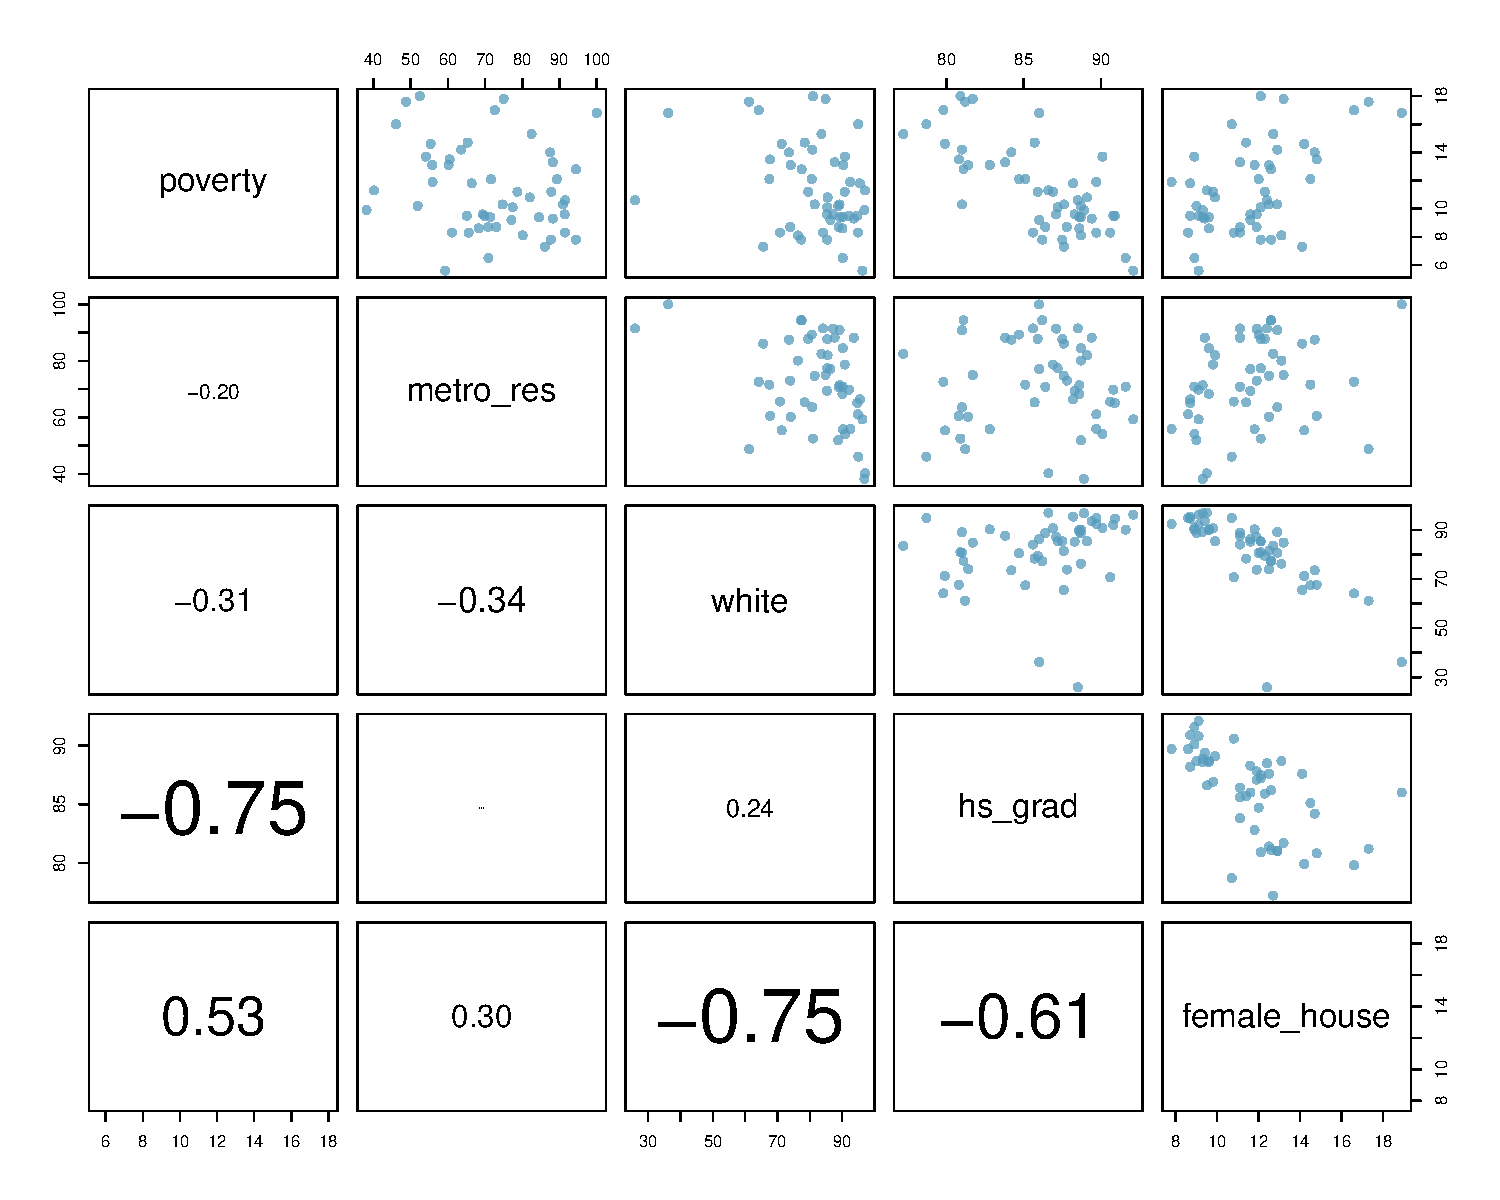
\includegraphics[width=0.9\textwidth]{9-1_intro_mlr/figures/poverty/poverty}
\end{center}

\end{frame}

%%%%%%%%%%%%%%%%%%%%%%%%%%%%%%%%%%%

\begin{frame}[fragile]
\frametitle{Predicting poverty using \% female householder}

\vspace{-0.25cm}

\begin{center}
\begin{tabular}{rrrrr}
  \hline
 & Estimate & Std. Error & t value & Pr($>$$|$t$|$) \\ 
  \hline
(Intercept) & 3.31 & 1.90 & 1.74 & 0.09 \\ 
  female\_house & 0.69 & 0.16 & 4.32 & 0.00 \\ 
   \hline
\end{tabular}
\end{center}
\twocol{0.5}{0.4}
{
\begin{center}
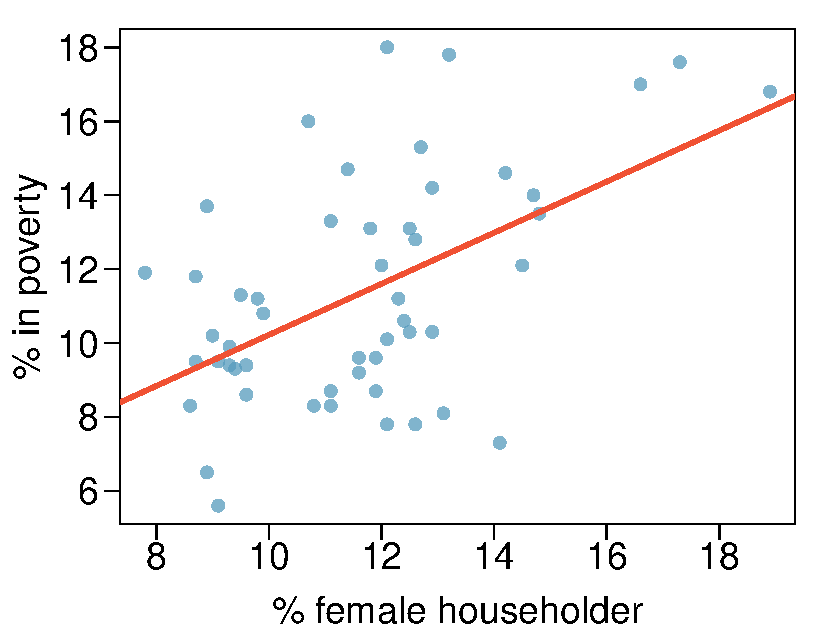
\includegraphics[width=\textwidth]{9-1_intro_mlr/figures/poverty/poverty_female_house}
\end{center}
}
{
\begin{align*}
R &= 0.53 \\
R^2 &= 0.53^2 = 0.28
\end{align*}
}

\end{frame}

%%%%%%%%%%%%%%%%%%%%%%%%%%%%%%%%%%%

\begin{frame}[fragile]
\frametitle{Another look at $R^2$}

$R^2$ can be calculated in three ways:

\pause

\begin{enumerate}

\item square the correlation coefficient of $x$ and $y$ {\small (how we have been calculating it)}

\pause

\item square the correlation coefficient of $y$ and $\hat{y}$

\pause

\item based on definition: 

\[ R^2 = \frac{\text{explained variability in }y}{\text{total variability in }y} \]

\end{enumerate}

\pause

Using \hl{ANOVA} we can calculate the explained variability and total variability in $y$.

\end{frame}


%%%%%%%%%%%%%%%%%%%%%%%%%%%%%%%%%%

\begin{frame}[fragile]
\frametitle{Sum of squares}

\vspace{-0.5cm}

{\small
\begin{center}
\begin{tabular}{lrrrrr}
  \hline
 & Df & Sum Sq & Mean Sq & F value & Pr($>$F) \\ 
  \hline
female\_house & 1 & 132.57 & 132.57 & 18.68 & 0.00 \\ 
  Residuals & 49 & 347.68 & 7.10 &  &  \\ 
   \hline
Total & 50 & 480.25 \\
   \hline
\end{tabular}
\end{center}
}

\pause

\begin{changemargin}{-1cm}{-1cm}
\begin{eqnarray*}
\text{Sum of squares of $y$: } SS_{Total} &=& \sum(y - \bar{y})^2 = 480.25 \orange{ {\footnotesize ~$\rightarrow$ total variability}} \\
\pause
%\text{Variance of $y$: } V(y) &=&  \frac{\sum(y - \bar{y})^2}{n-1} = 9.6 \\
%\pause
\text{Sum of squares of residuals: } SS_{Error} &=& \sum e_i^2 = 347.68 \orange{ { \footnotesize ~$\rightarrow$ unexplained variability}} \\
\pause
\text{Sum of squares of $x$: } SS_{Model} &=& SS_{Total} - SS_{Error} \orange{ {\footnotesize ~$\rightarrow$ explained variability}} \\
&=& 480.25 - 347.68 = 132.57
\end{eqnarray*}
\end{changemargin}

\pause

\[ R^2 = \frac{\text{explained variability}}{\text{total variability}} = \frac{132.57}{480.25} = 0.28 \green{~$\checkmark$} \]

\end{frame}

%%%%%%%%%%%%%%%%%%%%%%%%%%%%%%%%%%

\begin{frame}
\frametitle{Why bother?}

\dq{Why bother with another approach for calculating $R^2$ when we had a perfectly good way to calculate it as the correlation coefficient squared?}

\pause

\soln{\begin{itemize}
\item For single-predictor linear regression, having three ways to calculate the same value may seem like overkill. 
\item However, in multiple linear regression, we can't calculate $R^2$ as the square of the correlation between $x$ and $y$ because we have multiple $x$s. 
\item And next we'll learn another measure of explained variability, \hl{adjusted $R^2$}, that requires the use of the third approach, ratio of explained and unexplained variability. 
\end{itemize}}

\end{frame}

%%%%%%%%%%%%%%%%%%%%%%%%%%%%%%%%%%

\begin{frame}
\frametitle{Predicting poverty using \% female hh + \% white}


\begin{center}
\begin{tabular}{rrrrr}
  \hline
\hl{Linear model:}&  Estimate & Std. Error & t value & Pr($>$$|$t$|$) \\ 
  \hline
(Intercept) & -2.58 & 5.78 & -0.45 & 0.66 \\ 
  female\_house & 0.89 & 0.24 & 3.67 & 0.00 \\ 
  white & 0.04 & 0.04 & 1.08 & 0.29 \\ 
   \hline
\end{tabular}
\end{center}

\vspace{0.1cm}

\begin{center}
\begin{tabular}{lrrrrr}
  \hline
\hl{ANOVA:} & Df & Sum Sq & Mean Sq & F value & Pr($>$F) \\ 
  \hline
female\_house & 1 & 132.57 & 132.57 & 18.74 & 0.00 \\ 
  white & 1 & 8.21 & 8.21 & 1.16 & 0.29 \\ 
  Residuals & 48 & 339.47 & 7.07 &  &  \\ 
   \hline
Total & 50 &    480.25\\
   \hline
\end{tabular}
\end{center}

\pause

\[ R^2 = \frac{\text{explained variability}}{\text{total variability}} = \frac{132.57 + 8.21}{480.25} = 0.29 \]

\end{frame}

%%%%%%%%%%%%%%%%%%%%%%%%%%%%%%%%%%%

\begin{frame}
\frametitle{}

\dq{Does adding the variable \var{white} to the model add valuable information that wasn't provided by \var{female\_house}?}

\begin{center}
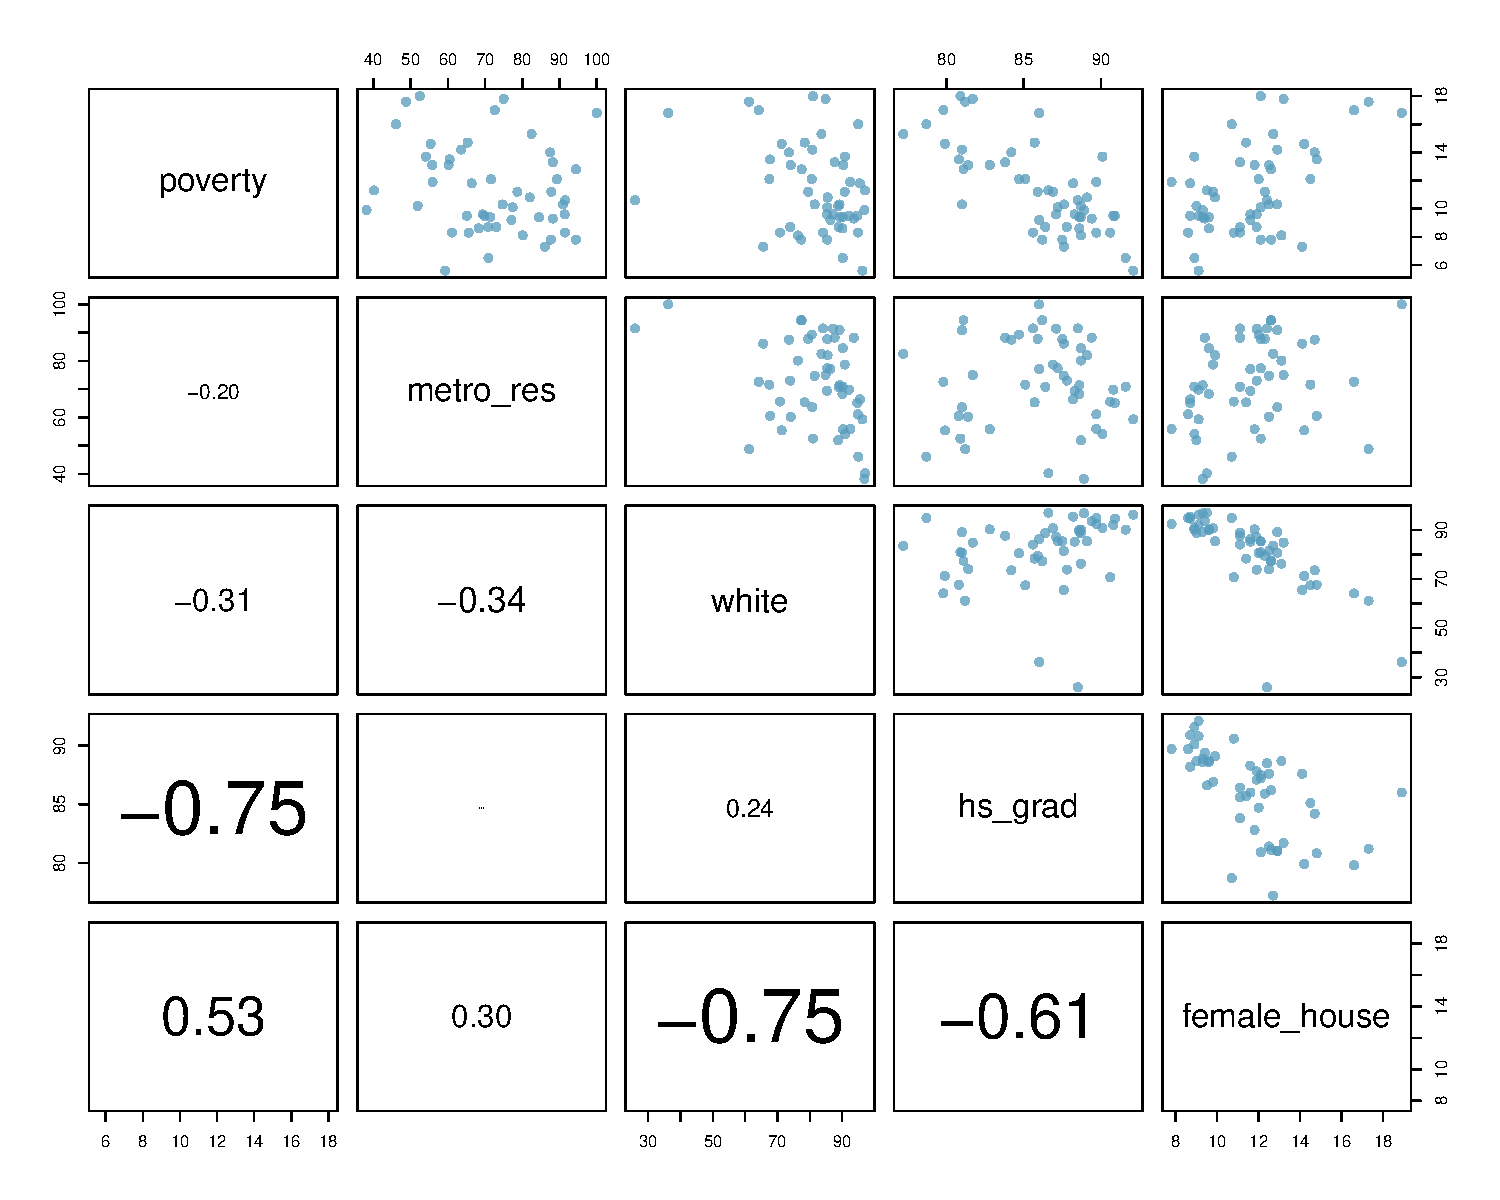
\includegraphics[width=0.8\textwidth]{9-1_intro_mlr/figures/poverty/poverty}
\end{center}

\end{frame}

%%%%%%%%%%%%%%%%%%%%%%%%%%%%%%%%%%%

\begin{frame}
\frametitle{Collinearity between explanatory variables}

\hl{poverty vs. \% female head of household}
\begin{center}
\begin{tabular}{rrrrr}
  \hline
 & Estimate & Std. Error & t value & Pr($>$$|$t$|$) \\ 
  \hline
(Intercept) & 3.31 & 1.90 & 1.74 & 0.09 \\ 
  female\_house & \only<1>{0.69} \only<2>{\orange{0.69}} & 0.16 & 4.32 & 0.00 \\ 
   \hline
\end{tabular}
\end{center}

$\:$ \\

\hl{poverty vs. \% female head of household and \% female hh}
\begin{center}
\begin{tabular}{rrrrr}
  \hline
 & Estimate & Std. Error & t value & Pr($>$$|$t$|$) \\ 
  \hline
(Intercept) & -2.58 & 5.78 & -0.45 & 0.66 \\ 
  female\_house & \only<1>{0.89} \only<2>{\orange{0.89}}  & 0.24 & 3.67 & 0.00 \\ 
  white & 0.04 & 0.04 & 1.08 & 0.29 \\   
   \hline
\end{tabular}
\end{center}

\end{frame}

%%%%%%%%%%%%%%%%%%%%%%%%%%%%%%%%%%%

\begin{frame}
\frametitle{Collinearity between explanatory variables (cont.)}

\begin{itemize}

\item Two predictor variables are said to be collinear when they are correlated, and this \hl{collinearity} complicates model estimation. \\
\Remember{Predictors are also called explanatory or \underline{independent} variables. Ideally, they would be independent of each other.}

\pause

\item We don't like adding predictors that are associated with each other to the model, because often times the addition of such variable brings nothing to the table. Instead, we prefer the simplest best model, i.e. \hl{parsimonious} model.

\pause

\item While it's impossible to avoid collinearity from arising in observational data, experiments are usually designed to prevent correlation among predictors.

\end{itemize}

\end{frame}

%%%%%%%%%%%%%%%%%%%%%%%%%%%%%%%%%%%
%
%
%\begin{frame}[fragile]
%\frametitle{F-test}
%
%ANOVA uses an F-test, which evaluates whether or not the $R^2$ is significant.
%
%
%
%\end{frame}
%
%%%%%%%%%%%%%%%%%%%%%%%%%%%%%%%%%%%%

\begin{frame}[fragile]
\frametitle{$R^2$ vs. adjusted $R^2$}

\renewcommand\arraystretch{1.25}
\begin{center}
\begin{tabular}{l | c  c}
			& $R^2$	& Adjusted $R^2$ \\
\hline
Model 1 (Single-predictor)	& 0.28	& 0.26 \\
Model 2 (Multiple)			& 0.29	& 0.26 	
\end{tabular}
\end{center}

\pause

\begin{itemize}

\item When \underline{any} variable is added to the model $R^2$ increases.

\pause

\item But if the added variable doesn't really provide any new information, or is completely unrelated, adjusted $R^2$ does not increase.

\end{itemize}



\end{frame}

%%%%%%%%%%%%%%%%%%%%%%%%%%%%%%%%%%%

\begin{frame}
\frametitle{Adjusted $R^2$}

\formula{Adjusted $R^2$}
{\[ R^2_{adj} = 1 - \pr{ \frac{ SS_{Error} }{ SS_{Total} } \times \frac{n - 1}{n - p - 1} } \]
where $n$ is the number of cases and $p$ is the number of predictors (explanatory variables) in the model.
}

\begin{itemize}

\item Because $p$ is never negative, $R^2_{adj}$ will always be smaller than $R^2$.

\item $R^2_{adj}$ applies a penalty for the number of predictors included in the model.

\item Therefore, we choose models with higher $R^2_{adj}$ over others.

\end{itemize}

\end{frame}

%%%%%%%%%%%%%%%%%%%%%%%%%%%%%%%%%%%

\begin{frame}
\frametitle{Calculate adjusted $R^2$}

\begin{center}
\begin{tabular}{lrrrrr}
  \hline
\hl{ANOVA:} & Df & Sum Sq & Mean Sq & F value & Pr($>$F) \\ 
  \hline
female\_house & 1 & 132.57 & 132.57 & 18.74 & 0.0001 \\ 
  white & 1 & 8.21 & 8.21 & 1.16 & 0.2868 \\ 
  Residuals & 48 & 339.47 & 7.07 &  &  \\ 
   \hline
Total & 50 &    480.25\\
   \hline
\end{tabular}
\end{center}

\begin{eqnarray*}
R^2_{adj} &=& 1 - \pr{ \frac{ SS_{Error} }{ SS_{Total} } \times \frac{n - 1}{n - p - 1} } \\
\pause
&=& 1 - \pr{ \frac{ 339.47 }{ 480.25 } \times \frac{51 - 1}{51 - 2 - 1} }   \\
\pause
&=& 1- \pr{ \frac{ 339.47 }{ 480.25 } \times \frac{50}{48} } \\
\pause
&=& 1 -  0.74 \\
\pause
&=& 0.26
\end{eqnarray*}

\end{frame}
